\section{Co-Design Aspects and Improvements}
\label{sec:codesign}

While above sections describe formulating initial design that satisfy design constraints, this section deals with obtaining an optimal one. For this purpose an automated script is built to search through the search space for obtaining an optimal solution. Following observations are made from the experiments.

\begin{enumerate}
	\item TDM frame size is inversely proportional to QOC. This is because less are the number of slots allocated to application more is the delay between successive samplings. This makes the system to respond slowly i.e higher settling time and lesser control. On the contrary when more slots are allocated to the application the delay between successive samplings is reduced and hence better control. But again when the resource utilization is high, i.e when almost all the slots are allocated to the application, it makes the system to respond rapidly and when adequate measures are not taken might result in an unstable system.
	
	\item A similar argument can be made for an increment in the slot size in the frame. Higher the slot size more is the frame size, higher the sampling period and lesser is the control. However in this case the resource utilization depends on the ratio of slot sizes P and C. Therefore lesser the slot size  doesn't necessarily imply a better QOC vs R graph.
	
	\item Placement of poles control the damping factor of the system effecting the rate at which the system responds. Closer the poles more rapid is the response. Poles very close might result in large overshoots driving the system unstable. This calls for a optimal pole selection, a trade-off between QOC and stability.
	
		\item Selecting more optimal poles requires less trial and error where it is possible to select for example initial value for all poles at 0.8 like before and then change the last value for the input current where it can help with the unstable input current experienced from those values. In Table \ref{tab:poles} the best choices from Table \ref{tab:list} were used and their poles optimized. When the poles were all at 0.8, some harmonics were visible in the input current and for poles all at 0.9 the settling time had increased considerably. Thus increasing the last three poles should affect the acceleration and the input current in such a way that they act more quickly and are less prone to fluctuation after settling.
		
		\begin{table}[htbp]
			\caption{}
			\begin{tabular}{rrlrrrrl}
				\toprule
				\multicolumn{1}{l}{C} & \multicolumn{1}{l}{P} & Poles & \multicolumn{1}{l}{Valid} & \multicolumn{1}{l}{QoC} & \multicolumn{1}{l}{R} & \multicolumn{1}{l}{$\dfrac{QoC}{R}$  } & Comment \\ 
				\midrule
				16000 & 8000 & [0.9 0.9 0.9 0.9 0.9] & 1 & 8.10 & 0.25 & 32.4 & \textcolor{red}{\textbf{“Bad” settling time}} \\ 
				16000 & 8000 & [0.8 0.8 0.85 0.9 0.9] & 1 & 11.59 & 0.25 & 46.4 & Good, but we could do better \\ 
				16000 & 8000 & [0.8 0.8 0.8 0.85 0.9] & 1 & 13.67 & 0.25 & 54.7 & \textcolor{blue}{\textbf{Optimal results}} \\ 
				16000 & 8000 & [0.8 0.8 0.8 0.8 0.8] & 1 & 18.34 & 0.25 & 73.3 & \textbf{Good, but: \textcolor{red}{Harmonics in input current}} \\ 
				\midrule
			\end{tabular}
			\label{tab:poles}
		\end{table}
\end{enumerate}

\begin{figure}[h]
	\begin{center}
		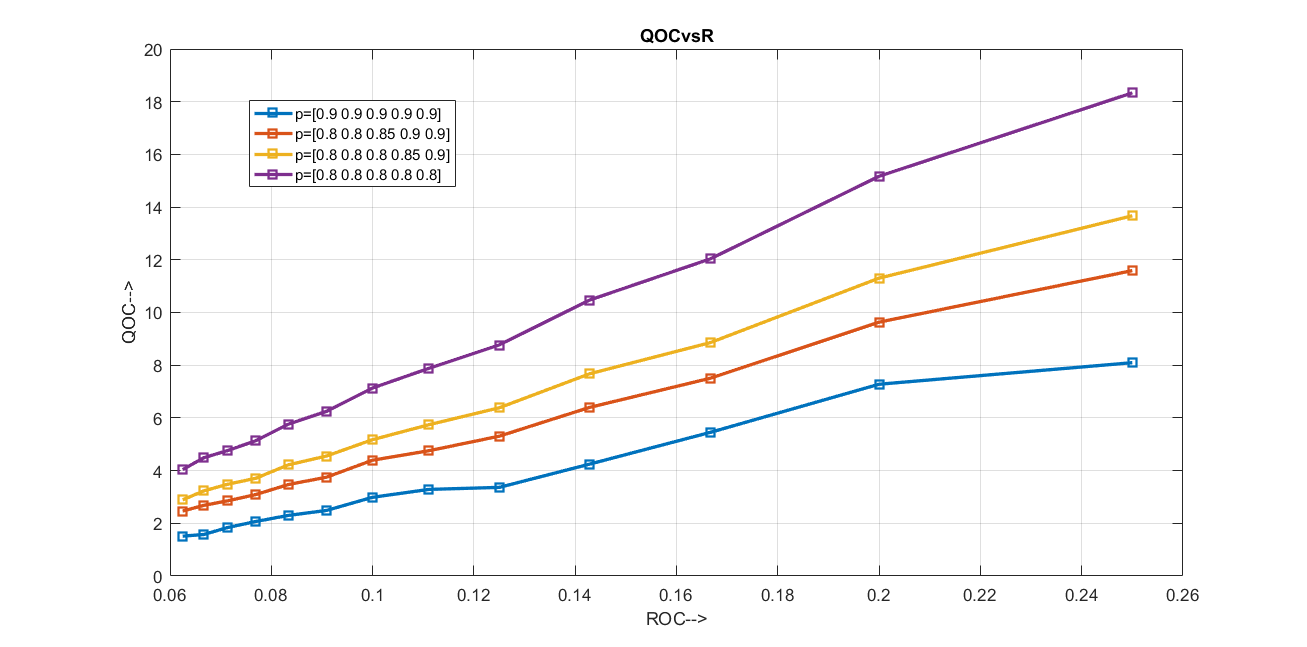
\includegraphics[width=\linewidth]{img/q2}
		\caption{QOC vs R for identical C and P. Poles are indicated in the legend and are according to Table \ref{tab:poles}}.
		\label{fig:qoc2}
	\end{center}
\end{figure}